% Appendix A

\chapter{Supplementary Material for \cref{selective_alignment}} % Main appendix title
\label{appendix-selal}

\section{Data and reference}
\label{subsec:meth_accessions}

The GENCODE v29 Human reference from
\url{https://www.gencodegenes.org/human/release_29.html} was used for all
experiments involving (simulated or experimental) human reads. The mouse
reference genome was obtained from
\url{ftp://ftp.ensembl.org/pub/release-91/fasta/mus_musculus/dna/Mus_musculus.GRCm38.dna.toplevel.fa.gz}
and the GTF was obtained from
\url{ftp://ftp.ensembl.org/pub/release-91/gtf/mus_musculus/Mus_musculus.GRCm38.91.gtf.gz}.
The VCF files for the SNPs and indels were obtained from
\url{ftp://ftp-mouse.sanger.ac.uk/REL-1410-SNPs_Indels/mgp.v4.snps.dbSNP.vcf.gz}
and
\url{ftp://ftp-mouse.sanger.ac.uk/REL-1410-SNPs_Indels/mgp.v4.indels.dbSNP.vcf.gz}
respectively. The list of 109 SRR, scripts to simulate synthetic reads, and the fasta
and true abundance files for 10 replicates of simulated data (gencode for human
and PWK for mouse) can be found at
\url{https://doi.org/10.5281/zenodo.3523437}.

\section{Decoy sequences}
\label{subsec:meth_decoy}

Alignment against the genome and transcriptome both have their advantages and
disadvantages, as discussed earlier. To avoid aligning genomic reads against
the transcriptome, without the need to index the complete genome, requires
finding regions with high sequence similarity between them. To obtain similar
sequences within a reference, we mapped the spliced transcript sequences against
a version of the genome where all exon segments were hard-masked (i.e.\@
replaced with \texttt{N}). We performed this mapping using
MashMap~\citep{jain2018fast}, with a segment size 500 and minimum percent
identity of 80\%. The sequence similar regions were merged (per-chromosome)
using BedTools~\citep{quinlan2010bedtools} and concatenated, giving a decoy
sequence for each chromosome. These decoys were then included during the
\salmon indexing phase, as described below. A script to obtain these decoy
sequences for any reference, given the genome, transcriptome, and annotation
is available at: \url{https://github.com/COMBINE-lab/SalmonTools/blob/master/scripts/generateDecoyTranscriptome.sh}.

\section{Tools}
\label{subsec:commands}
We used \salmon v0.15.0 for quasi-mapping and \salmon v1.0 for \hsa and \saf, Bowtie2 version 2.3.4.3, STAR version 2.6.1b, tximport
version 1.12.3, DESeq2 version 1.24.0, kallisto version 0.45.1, edgeR version 3.24.3, limma version 3.38.3, 
RSEM version 1.2.28, Trim Galore version 0.5.0, bedtools v2.28.0, sleuth version 0.30.0 and
MashMap v2.0. All simulated datasets were generated using Polyester version 1.18.0.

For quality trimming the reads we used the following command:
\raggedright
\begin{enumerate}
\item \textbf{trim\_galore} \texttt{-q 20 --phred33 --length 20 --paired <fastq file>}
\end{enumerate}

For indexing, we use the following extra command line arguments, along with the regular
indexing and threads parameters:
\begin{enumerate}
\item \textbf{STAR} \texttt{--genomeFastaFiles <fasta file> --sjdbGTFfile <gtf file> --sjdbOverhang 100}
\item \textbf{Bowtie2} \texttt{default}
\item \textbf{salmon} \texttt{-k 23 --keepDuplicates}
\item \textbf{kallisto} \texttt{-k 23}
\end{enumerate}

For quantification, we use the following extra command line, along with regular
index and threads, with each tools we compare against:
\raggedright
\begin{enumerate}
	\item \textbf{SA and SAF} \texttt{--mimicBT2 --useEM}
	\item \textbf{quasi} \texttt{--rangeFactorizationBins 4 --discardOrphansQuasi --useEM --noSA}
	\item \textbf{Bowtie2} \texttt{--sensitive -k 200 -X 1000 --no-discordant --no-mixed --gbar 1}
	\item \textbf{Bowtie2\_strict} \texttt{--sensitive --dpad 0 --gbar 99999999 --mp 1,1
	  --np 1 --score-min L,0,-0.1 --no-mixed --no-discordant -k 200 -I 1 -X 1000}
	\item \textbf{Bowtie2\_RSEM} \texttt{--sensitive --dpad 0 --gbar 99999999 --mp 1,1
	  --np 1 --score-min L,0,-0.1 --no-mixed --no-discordant -k 200 -I 1 -X 1000}
	\item \textbf{STAR} \texttt{--outFilterType BySJout --alignSJoverhangMin 8 
	--outFilterMultimapNmax 20 --alignSJDBoverhangMin 1 --outFilterMismatchNmax 999
	--outFilterMismatchNoverReadLmax 0.04 --alignIntronMin 20 --alignIntronMax 1000000 
	--alignMatesGapMax 1000000 --readFilesCommand zcat --outSAMtype BAM Unsorted 
	--quantMode TranscriptomeSAM --outSAMattributes NH HI AS NM MD 
	--quantTranscriptomeBan Singleend}
	\item \textbf{STAR\_strict} \texttt{--outFilterType BySJout --alignSJoverhangMin 8 
	--outFilterMultimapNmax 20 --alignSJDBoverhangMin 1 --outFilterMismatchNmax 999
	--outFilterMismatchNoverReadLmax 0.04 --alignIntronMin 20 --alignIntronMax 1000000 
	--alignMatesGapMax 1000000 --readFilesCommand zcat --outSAMtype BAM Unsorted 
	--quantMode TranscriptomeSAM --outSAMattributes NH HI AS NM MD
	--quantTranscriptomeBan IndelSoftclipSingleend}
	\item \textbf{STAR\_RSEM} \texttt{--outFilterType BySJout --alignSJoverhangMin 8 
	--outFilterMultimapNmax 20 --alignSJDBoverhangMin 1 --outFilterMismatchNmax 999
	--outFilterMismatchNoverReadLmax 0.04 --alignIntronMin 20 --alignIntronMax 1000000 
	--alignMatesGapMax 1000000 --readFilesCommand zcat --outSAMtype BAM Unsorted 
	--quantMode TranscriptomeSAM --outSAMattributes NH HI AS NM MD
	--quantTranscriptomeBan IndelSoftclipSingleend}
	\item \textbf{RSEM} \texttt{default}
	\item \textbf{kallisto} \texttt{default} or \texttt{--rf-stranded} as appropriate
\end{enumerate}

\begin{table}[h!]
 \centering
 \begin{tabular}{ccccc}
   \hline
   				& \multicolumn{1}{p{1.5cm}}{\centering Genome indexed} & \multicolumn{1}{p{1.5cm}}{\centering Alignment scoring} &
				\multicolumn{1}{p{1.5cm}}{\centering Indels allowed} &
				\multicolumn{1}{p{2cm}}{\centering Quantification method} \\ \hline
      Bowtie2		& \xmark & \cmark & \cmark & \salmon \\
      Bowtie2\_strict	& \xmark & \cmark & \xmark & \salmon \\
      Bowtie2\_RSEM	& \xmark & \cmark & \xmark & RSEM \\
      STAR			& \cmark & \cmark & \cmark  & \salmon \\
      STAR\_strict	& \cmark & \cmark & \xmark  & \salmon \\
      STAR\_RSEM	& \cmark & \cmark & \xmark  & RSEM \\
      quasi			& \xmark & \xmark & \cmark  & \salmon \\
      \hsa			& \xmark$^{*}$ & \cmark$^{**}$ & \cmark & \salmon \\
      \saf			& \cmark & \cmark$^{**}$ & \cmark & \salmon \\
   \hline
\end{tabular}
 \caption{Various factors altered under each pipeline. *Here, under \hsa, only
  regions of the genome that are sequence similar to the transcriptome are indexed, but not
  the whole genome. Refer to~\Cref{subsec:meth_decoy} for further details on how the sequences are obtained.
  **While \hsa and \saf produce alignment scores, they do not perform backtracing or reconstruct the edit
  operations that were used to obtain the optimal alignment score.}
 \label{tab:methods}
\end{table}

\begin{figure}[h!]
  \centering
  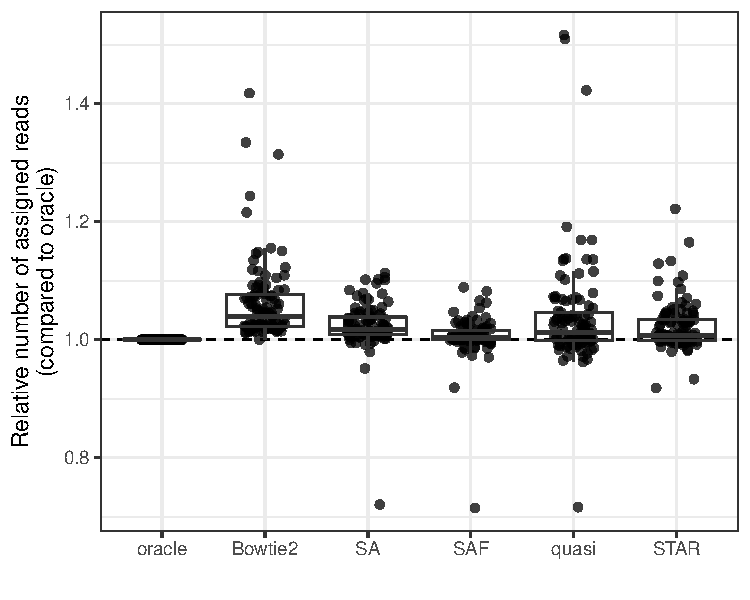
\includegraphics[width=\linewidth]{selal/mrate.pdf}
  \caption{Mapping rates of different methods, relative to oracle, for 109 experimental samples.}
  \label{fig:mrate}
\end{figure}

\begin{table}[h!]
 \centering
 \begin{tabular}{ccccccc}
   \hline
         & Oracle & Bowtie2 & SAF & \hsa & quasi & STAR\\ \hline
 Oracle & 1.000/0.000 & $\numprint{0.858495}$/$\numprint{0.053736}$ & $\numprint{0.919992}$/$\numprint{0.028552}$ & $\numprint{0.873352}$/$\numprint{0.045867}$& $\numprint{0.843022}$/$\numprint{0.053193}$& $\numprint{0.889439}$/$\numprint{0.039311}$\\
 Bowtie2 & -- & 1.000/0.000 & $\numprint{0.817429}$/$\numprint{0.063481}$ & $\numprint{0.863387}$/$\numprint{0.038621}$ & $\numprint{0.783076}$/$\numprint{0.067582}$ & $\numprint{0.790747}$/$\numprint{0.068541}$ \\
 SAF & -- & -- & 1.000/0.000 & $\numprint{0.906522}$/$\numprint{0.052332}$ & $\numprint{0.864903}$/$\numprint{0.049687}$ & $\numprint{0.909014}$/$\numprint{0.023030}$\\
 \hsa & -- & -- & -- & 1.000/0.000 & $\numprint{0.829317}$/$\numprint{0.063462}$ & $\numprint{0.836573}$/$\numprint{0.058815}$ \\
 quasi &  -- & --  & -- & -- & 1.000/0.000 & $\numprint{0.858436}$/$\numprint{0.052212}$\\
 STAR &  -- & --  & -- & -- & -- & 1.000/0.000 \\
 \hline
\end{tabular}
 \caption{Mean/standard deviation of Spearman correlation between all methods on $40$ single-cell experimental datasets after 
 removing short transcripts with length $<300$. }
 \label{tab:withoutshortsc}
\end{table}

\begin{table}[h!]
 \centering
 \begin{tabular}{ccccccc}
   \hline
         & Oracle & Bowtie2 & SAF & \hsa & quasi & STAR\\ \hline
 Oracle & 1.000/0.000 & $\numprint{0.949207}$/$\numprint{0.022744}$ & $\numprint{0.970706}$/$\numprint{0.008334}$ & $\numprint{0.954241}$/$\numprint{0.013979}$& $\numprint{0.907292}$/$\numprint{0.031031}$& $\numprint{0.962499}$/$\numprint{0.012450}$\\
 Bowtie2 & -- & 1.000/0.000 & $\numprint{0.940024}$/$\numprint{0.026027}$ & $\numprint{0.961004}$/$\numprint{0.017293}$ & $\numprint{0.901297}$/$\numprint{0.034042}$ & $\numprint{0.919557}$/$\numprint{0.025325}$ \\
 SAF & -- & -- & 1.000/0.000 & $\numprint{0.971655}$/$\numprint{0.015035}$ & $\numprint{0.913026}$/$\numprint{0.030584}$ & $\numprint{0.954660}$/$\numprint{0.011279}$\\
 \hsa & -- & -- & -- & 1.000/0.000 & $\numprint{0.913908}$/$\numprint{0.028960}$ & $\numprint{0.932170}$/$\numprint{0.016787}$ \\
 quasi &  -- & --  & -- & -- & 1.000/0.000 & $\numprint{0.903269}$/$\numprint{0.029167}$\\
 STAR &  -- & --  & -- & -- & -- & 1.000/0.000 \\
 \hline
\end{tabular}
 \caption{Mean/standard deviation of Spearman correlation between all methods on $69$ bulk experimental datasets after 
 removing short transcripts with length $<300$. }
 \label{tab:withoutshortbulk}
\end{table}

\begin{figure}[h!]
    \centering
     \begin{subfigure}[t]{0.49\textwidth}
     \centering
  	  	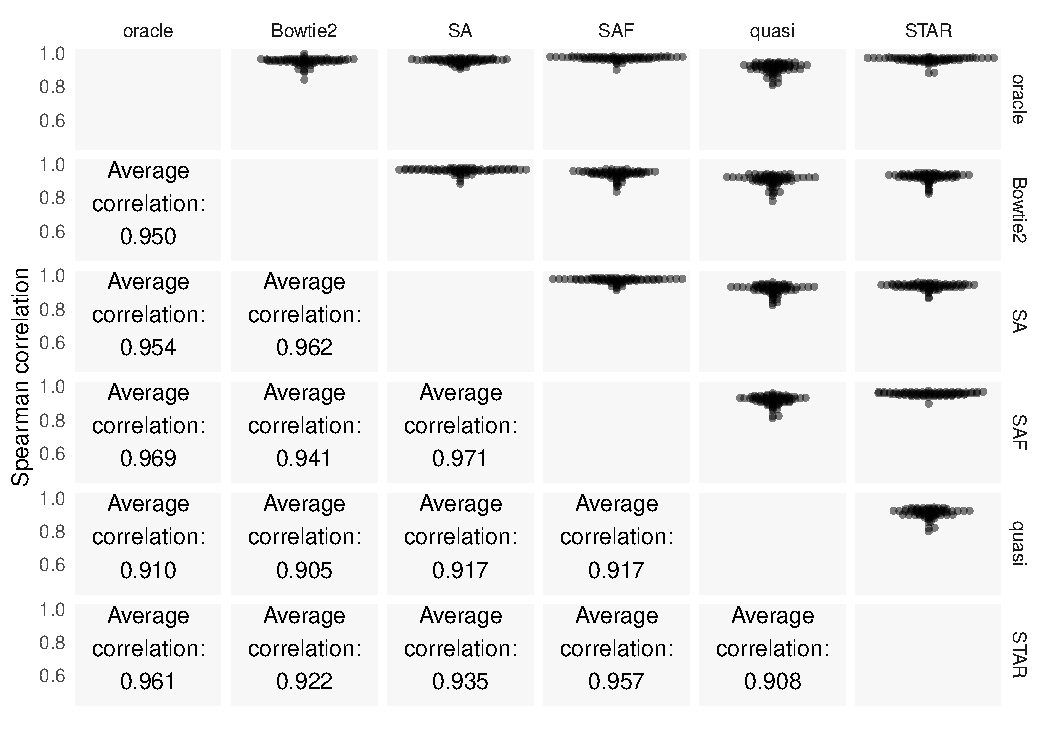
\includegraphics[width=\linewidth]{selal/bulk_pairwise_correlations_real_data_count.pdf}
		\caption{Bulk}
    \end{subfigure}
     \begin{subfigure}[t]{0.49\textwidth}
     \centering
  	  	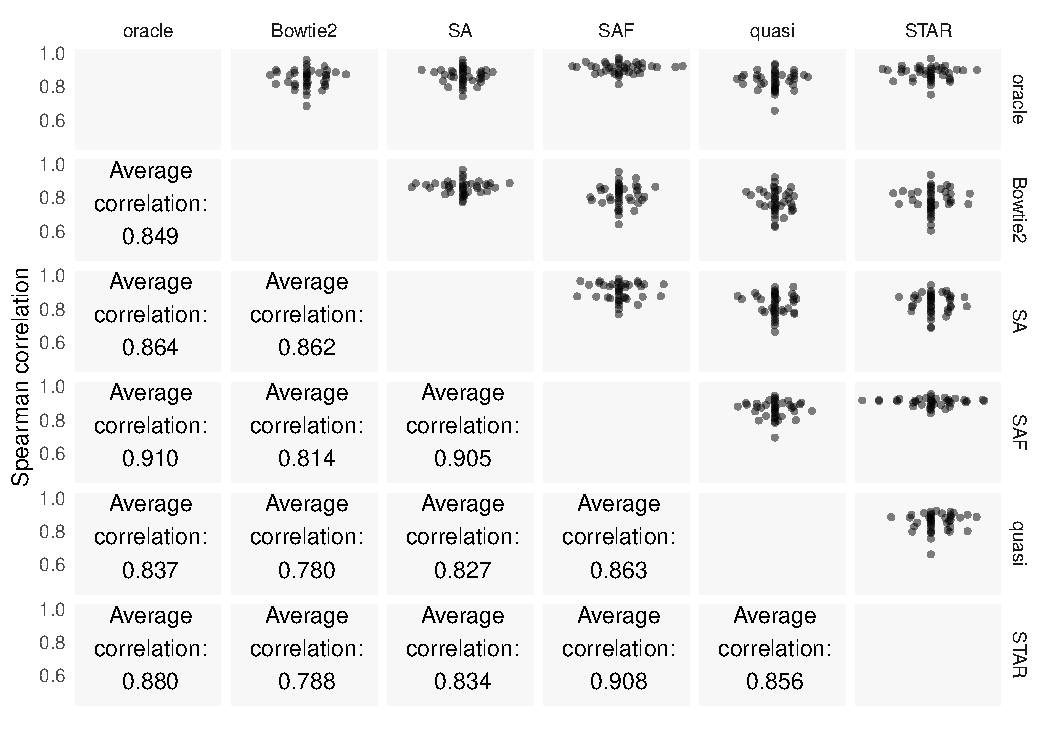
\includegraphics[width=\linewidth]{selal/singlecell_pairwise_correlations_real_data_count.pdf}
		\caption{Single-cell}
    \end{subfigure}   
     \caption{The upper triangle of the matrix shows swarm plots of pairwise correlations of read counts predicted by
       the different approaches on the experimental samples. The bottom half 
       shows the average Spearman correlations between methods across the $109$ bulk and single-cell samples.}
    \label{fig:swarmcount}
\end{figure}

\begin{figure}[h!]
    \centering
    \begin{subfigure}[t]{0.7\textwidth}
        \centering
  	  	 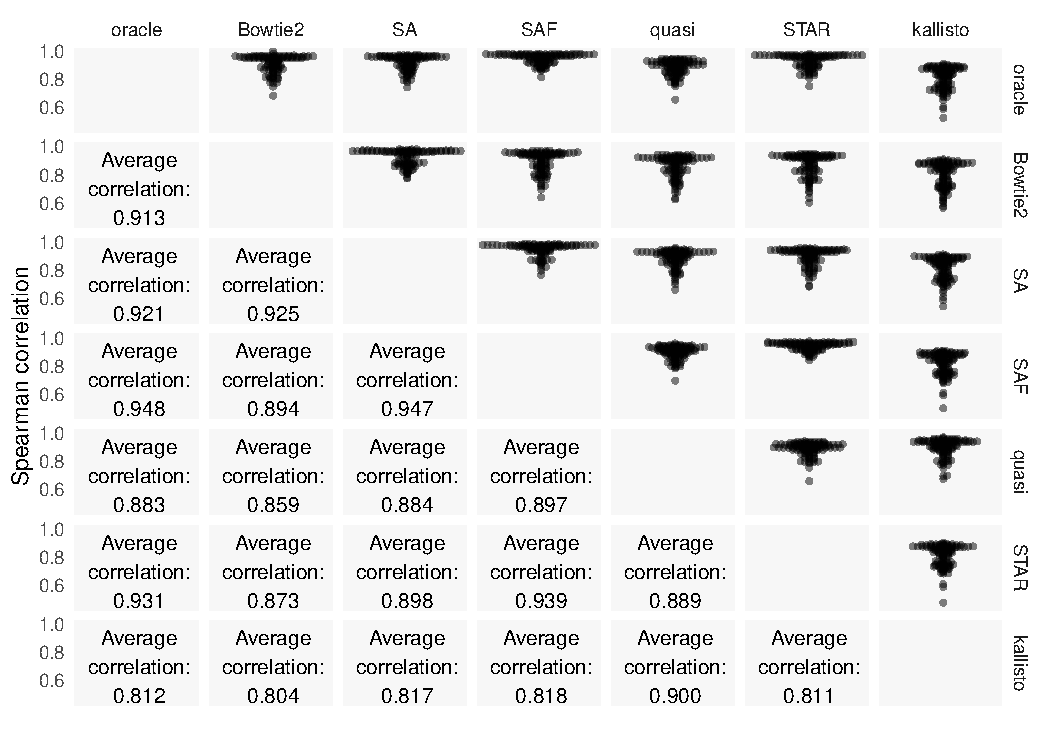
\includegraphics[width=\linewidth]{selal/pairwise_correlations_real_data_kallisto.pdf}
		\caption{}
    \end{subfigure}
    ~ 
    \begin{subfigure}[t]{0.7\textwidth}
        \centering
  	  	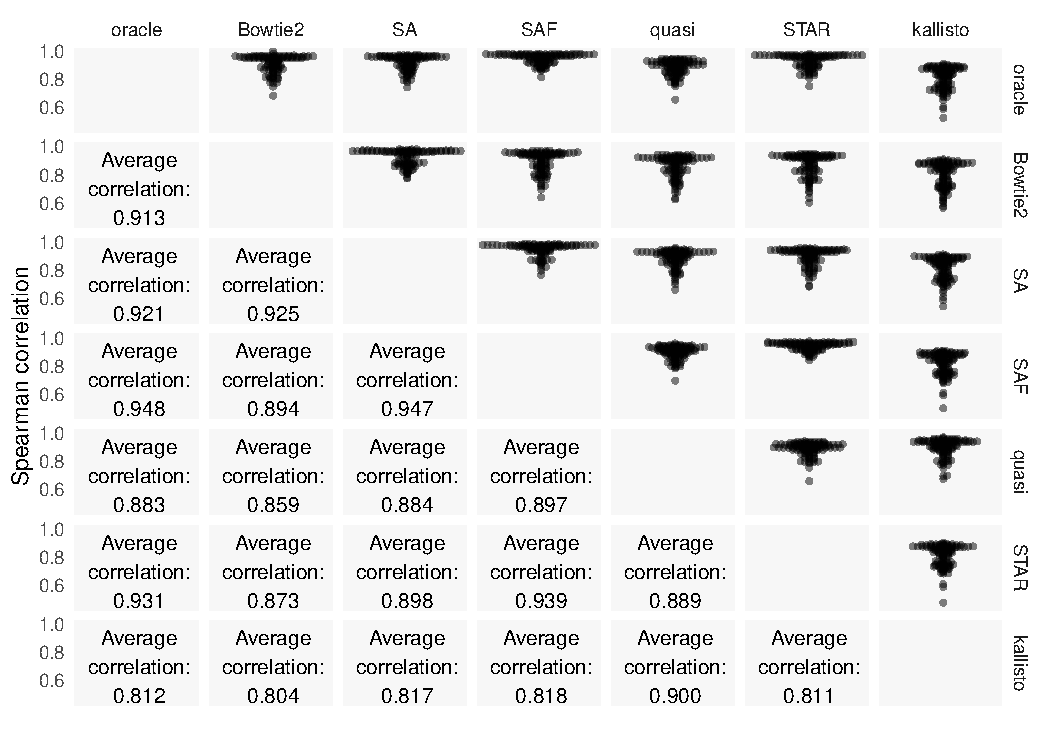
\includegraphics[width=\linewidth]{selal/pairwise_correlations_real_data_kallisto.pdf}
		\caption{}
    \end{subfigure}
    \caption{The top half of each matrix shows swarm plots of the pairwise correlations using count (a) and TPM (b) values
        predicted by the different approaches on the experimental samples. The
        bottom half shows the average Spearman correlations between methods
        across the $109$ samples. Note that the quantification method for each
        pipeline is the same, except \kallisto, where both the mapping and
        quantification algorithms are different. Hence, while other methods
        disallow orphaned reads and dovetailed mappings, the \kallisto output
        will include them, which may explain, in part, the increased divergence
        from the alignment-based methods.}
    \label{fig:kallisto}
\end{figure}

\begin{figure}[t!]
    \centering
    \begin{subfigure}[t]{0.45\textwidth}
        \centering
	    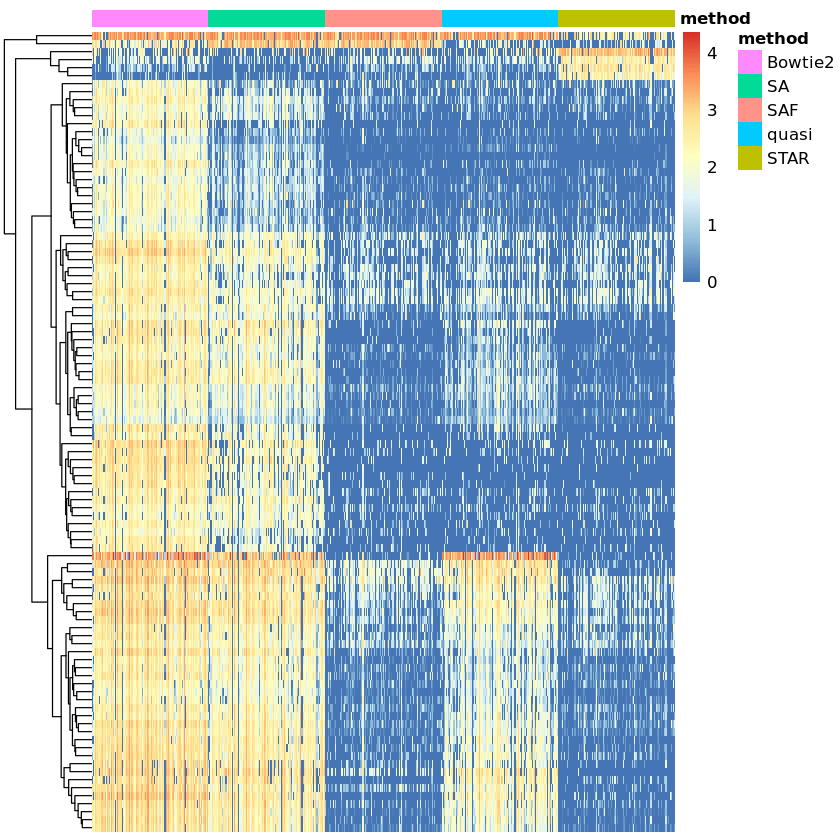
\includegraphics[width=\linewidth]{selal/heatmap_100.png}
	    \caption{}
    \end{subfigure}
    ~
    \begin{subfigure}[t]{0.45\textwidth}
        \centering
	    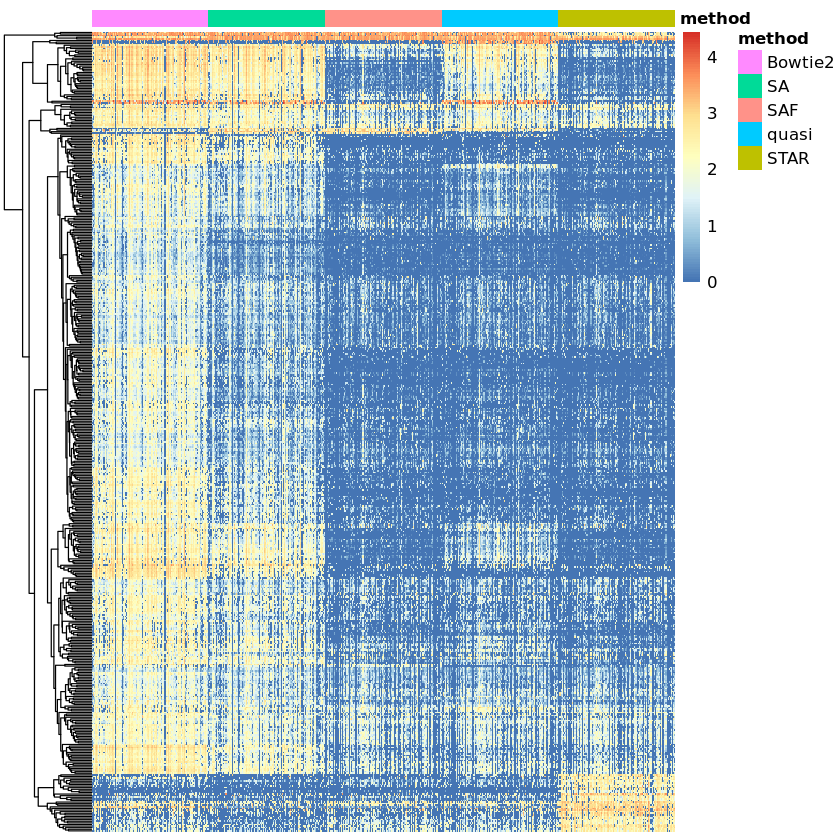
\includegraphics[width=\linewidth]{selal/heatmap_500.png}
	    \caption{}
    \end{subfigure}
    ~
     \begin{subfigure}[t]{0.45\textwidth}
     \centering
	    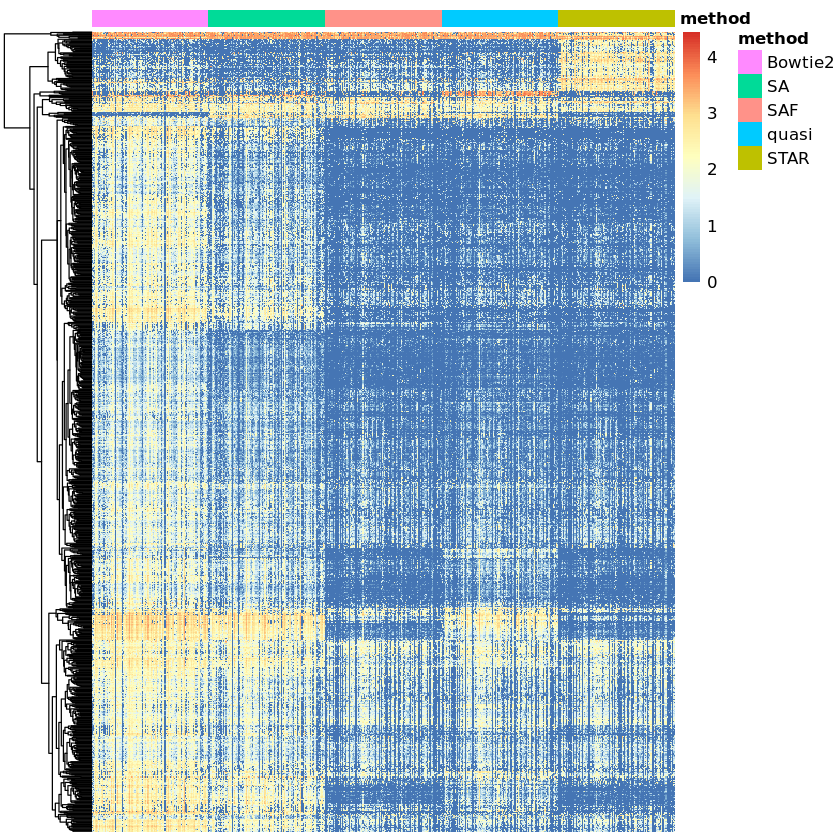
\includegraphics[width=\linewidth]{selal/heatmap_1k.png}
	    \caption{}
    \end{subfigure}
    \caption{The $\log_2(\text{CPM})$ for 109 samples grouped by
      method for the top 100 (a), 500 (b), and 1000 (c) differential transcripts. 
      Limma-trend was used with \texttt{scaledTPM} counts 
	(generating counts from per-sample TPMs by scaling to the library size) via
	tximport~\citep{soneson2015differential}, with a \texttt{prior.count} of
	3, and using a design of \texttt{$\sim$sample + method}. An F-statistic was
	generated by specifying coefficients representing differences among the methods
	and the top transcripts chosen using the F-test p-value.}
      \label{fig:heatmap}
\end{figure}

\begin{figure}[h!]
    \centering
     \begin{subfigure}[t]{0.49\textwidth}
     \centering
  	  	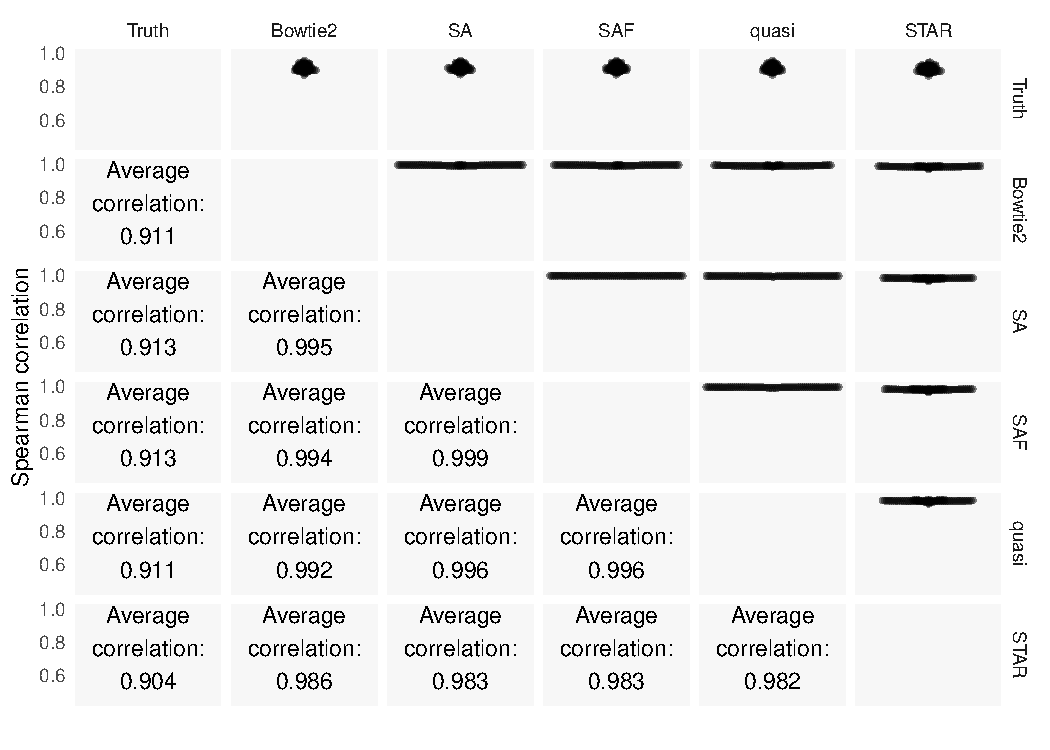
\includegraphics[width=\linewidth]{selal/bulk_pairwise_correlations_sim_data.pdf}
		\caption{Bulk}
    \end{subfigure}
     \begin{subfigure}[t]{0.49\textwidth}
     \centering
  	  	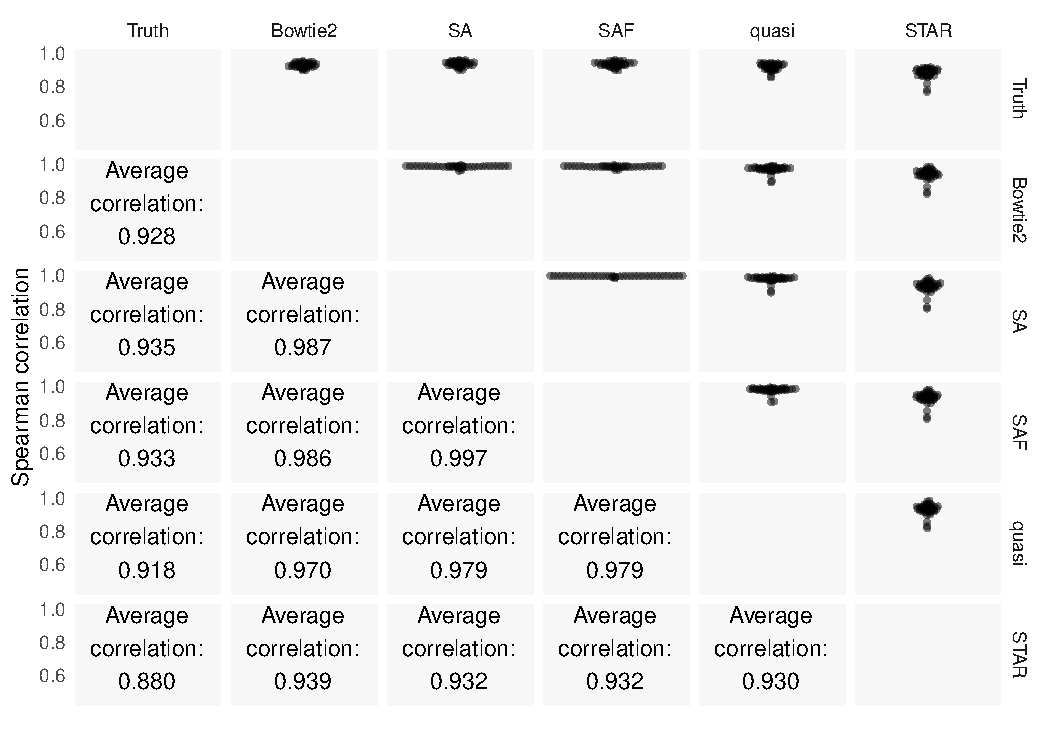
\includegraphics[width=\linewidth]{selal/singlecell_pairwise_correlations_sim_data.pdf}
		\caption{Single-cell}
    \end{subfigure}
     \caption{The top half of the matrix shows swarm plots of the pairwise correlations of TPM 
	 values predicted by the
       different approaches with each other and with the ground truth abundances
       on the simulated samples. The bottom half shows the average Spearman
       correlations between the different approaches across the $109$ samples.
       The expected effective length of each transcript was computed according
       to the true fragment length distribution. Given the true fragment counts
       and expected effective lengths, the TPM is computed as in~\citet{rsem}.}
    \label{fig:swarmsimTPM}
\end{figure}

\begin{figure}[ht!]
    \centering
    \begin{subfigure}[t]{0.49\textwidth}
        \centering
  	  	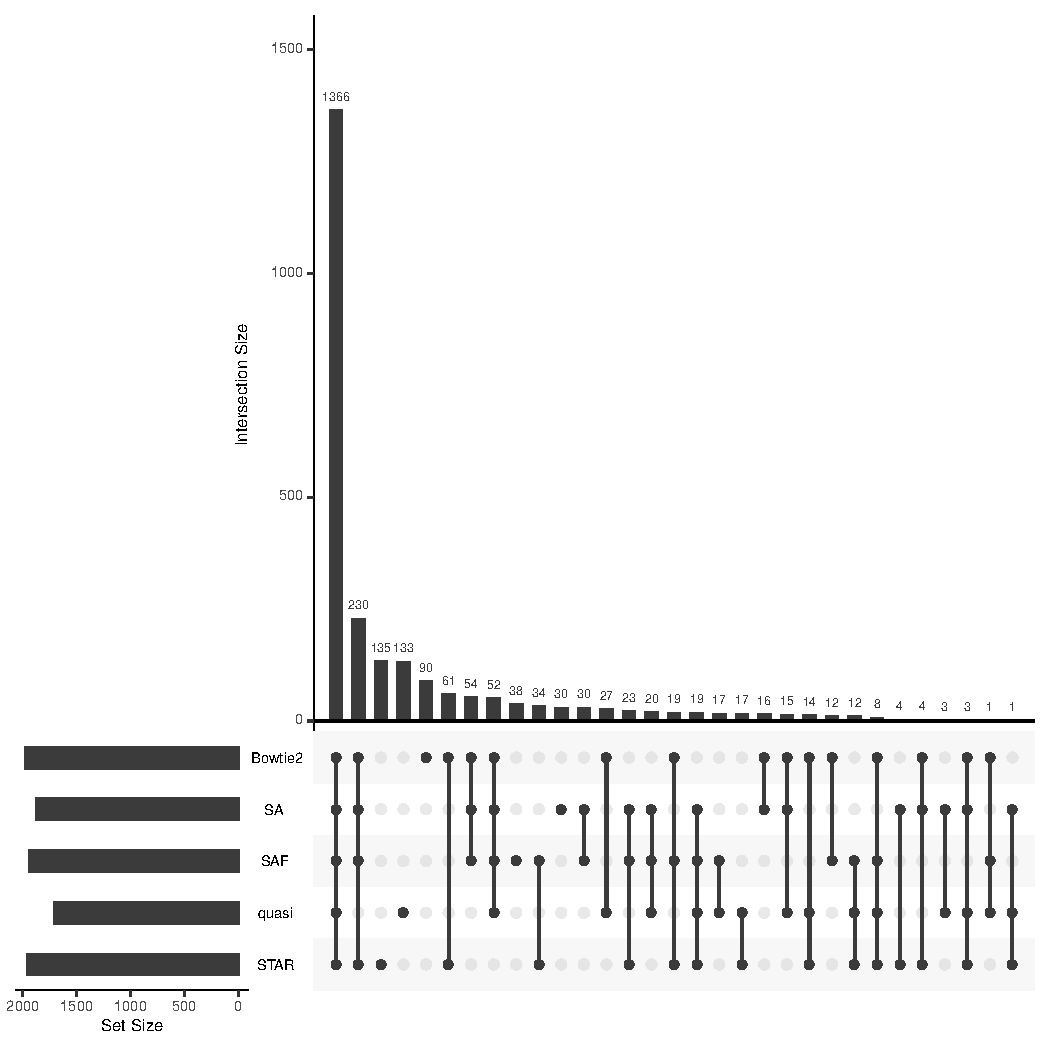
\includegraphics[width=\linewidth]{selal/alsfdr5.pdf}
		\caption{}
    \end{subfigure}
    ~ 
    \begin{subfigure}[t]{0.49\textwidth}
        \centering
  	  	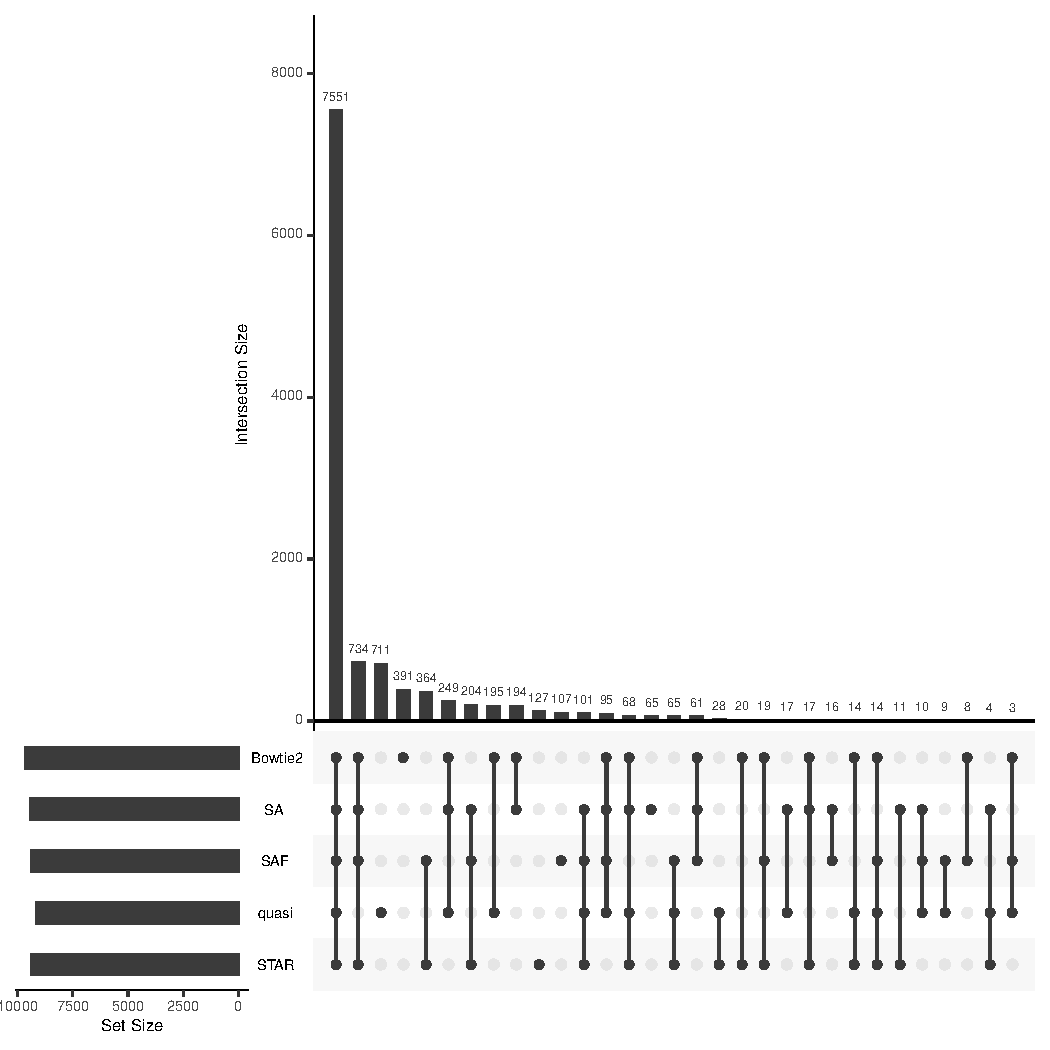
\includegraphics[width=\linewidth]{selal/hsvfdr5.pdf}
		\caption{}
    \end{subfigure}
    ~
    \begin{subfigure}[t]{0.49\textwidth}
        \centering
  	  	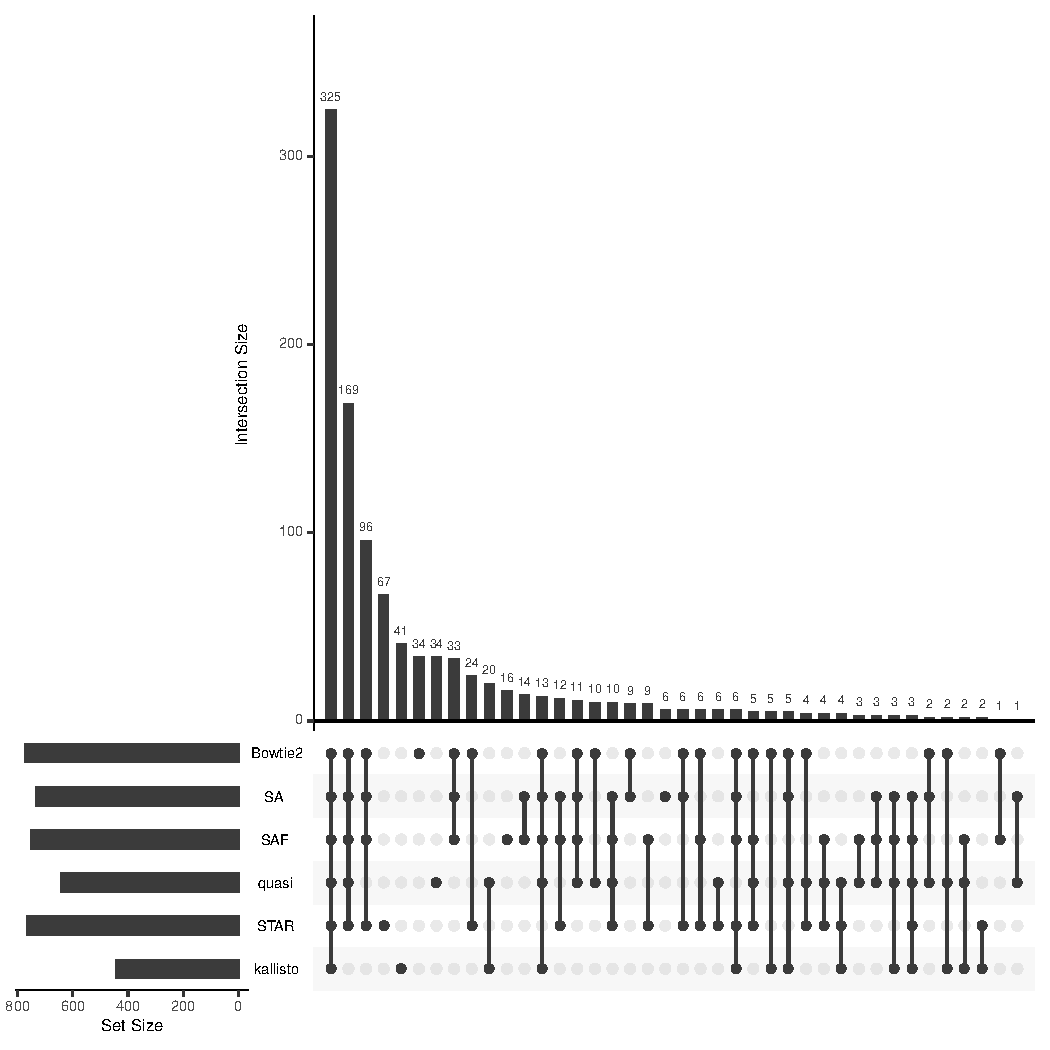
\includegraphics[width=\linewidth]{selal/alskal.pdf}
		\caption{}
    \end{subfigure}
    ~ 
    \begin{subfigure}[t]{0.49\textwidth}
        \centering
  	  	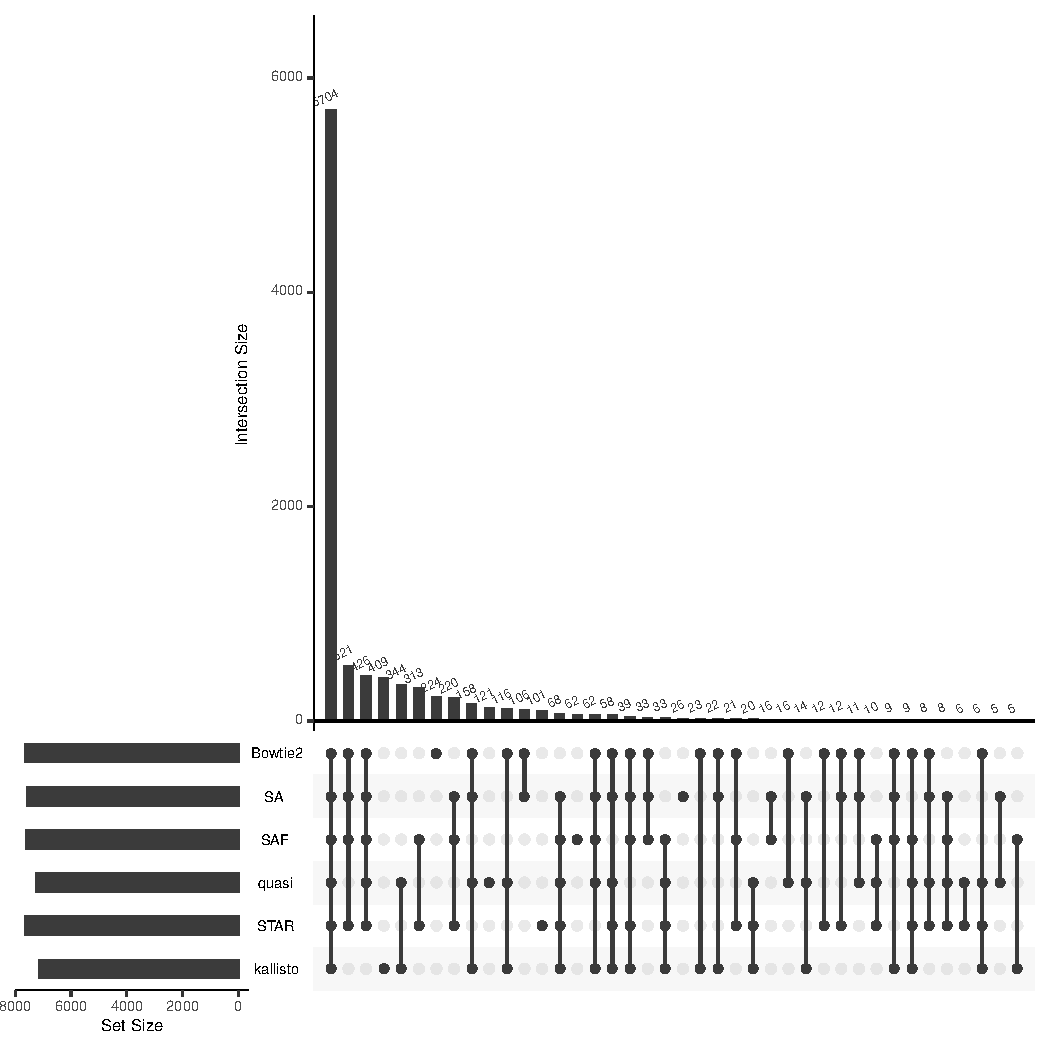
\includegraphics[width=\linewidth]{selal/hsvkal.pdf}
		\caption{}
    \end{subfigure}
    \caption{Comparison of sets of differentially expressed genes, and their overlaps, computed using each method.
    Figures (a) and (b) shows the results for the two datasets when filtered at an FDR of $0.05$ and 
    (c) and (d) shows the results at FDR $0.01$ after including kallisto as an additional lightweight mapping approach.}
    \label{fig:suppdge}
\end{figure}

\begin{figure}[ht!]
    \centering
    \begin{subfigure}[t]{0.49\textwidth}
        \centering
  	  	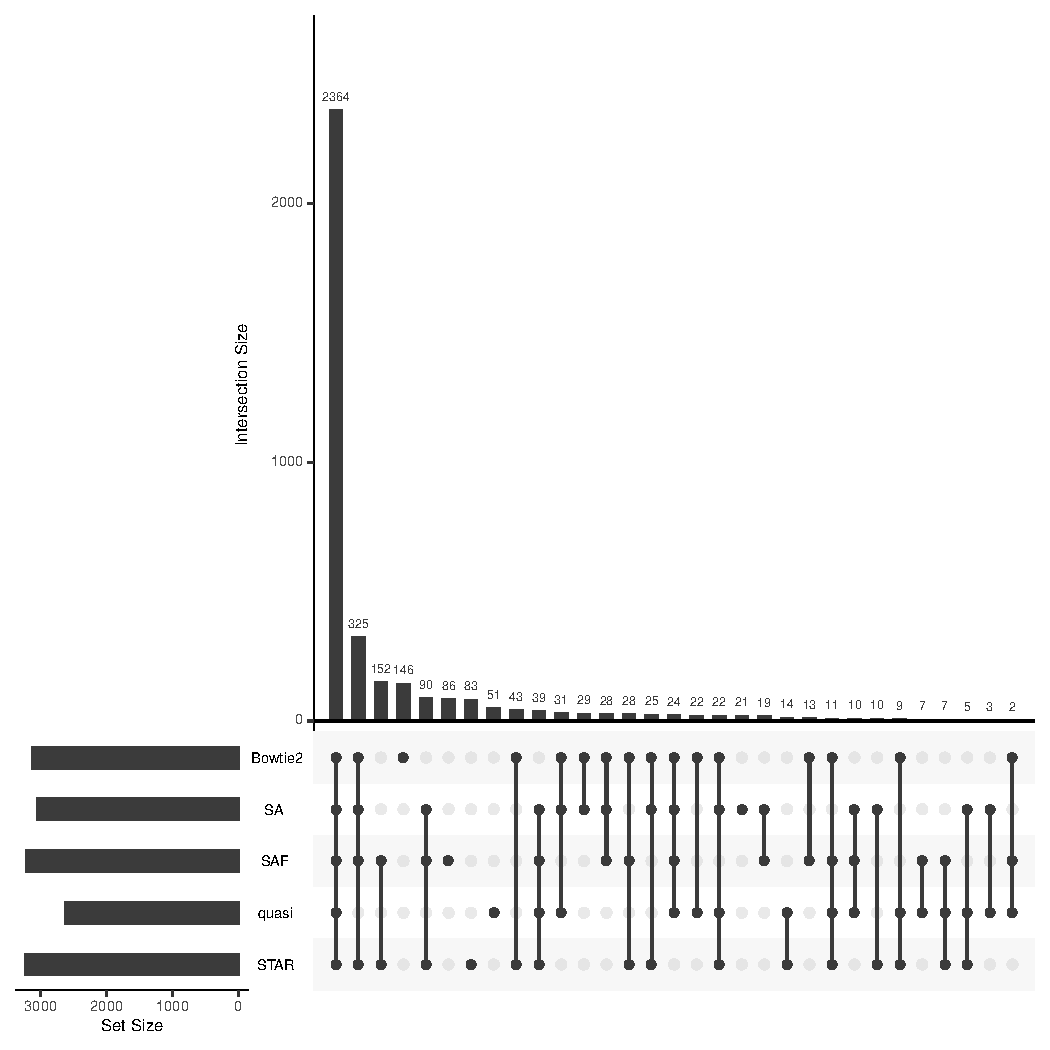
\includegraphics[width=\linewidth]{selal/zikafdr5.pdf}
		\caption{}
    \end{subfigure}
    ~ 
    \begin{subfigure}[t]{0.49\textwidth}
        \centering
  	  	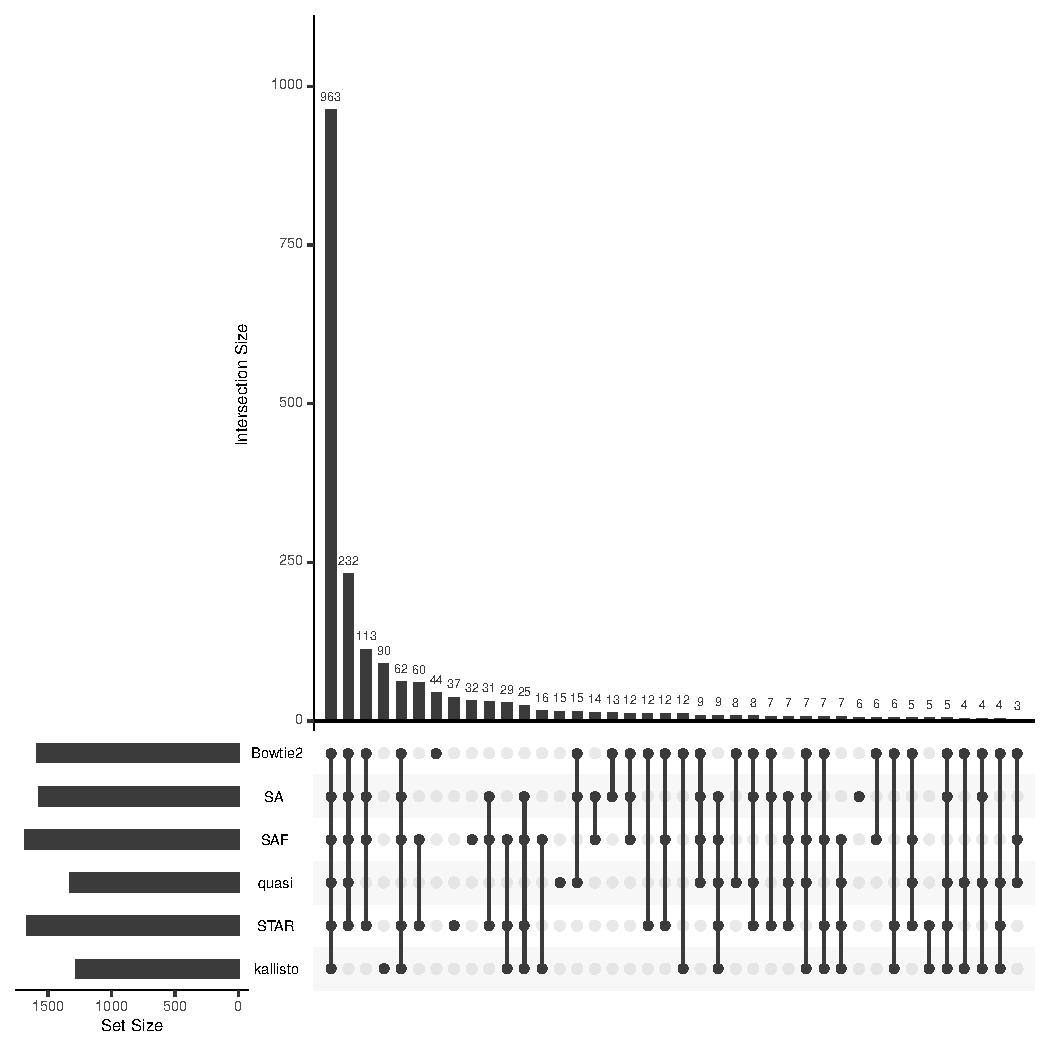
\includegraphics[width=\linewidth]{selal/zikakal.pdf}
		\caption{}
    \end{subfigure}
    \caption{Comparison of sets of differentially expressed transcripts, and their overlaps, computed using each method.
    Figure (a) shows the results when filtered at an FDR of $0.05$ and (b) shows the results at FDR $0.01$ after including kallisto as 
    an additional lightweight mapping approach.}
    \label{fig:suppdte}
\end{figure}